\subsection{Preprocessing techniques}
In this section, we have implemented the preprocessing techniques we described above to different level of attacks, to be more specific the $\epsilon$ in FGSM attack. We then plot the accuracy of our net, with various values of parameters in different techniques.

\subsubsection{Bit-Depth Reduction}

\begin{figure}[h!]
	\centering
	\begin{subfigure}{.4\textwidth}
		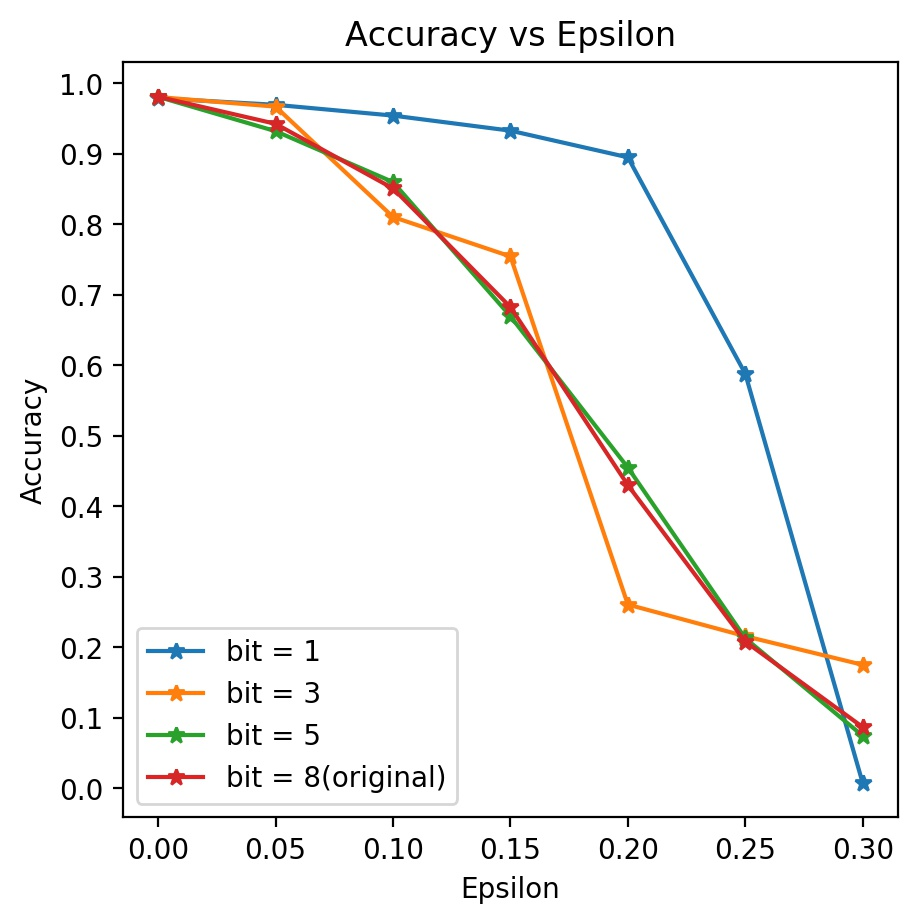
\includegraphics[width=\textwidth]{pretrained_Accuracy_vs_Epsilon_db.jpg}
		\caption{pretrained model}
		\label{fig: bit-depth reduction pre}
	\end{subfigure}
	\begin{subfigure}{.4\textwidth}
		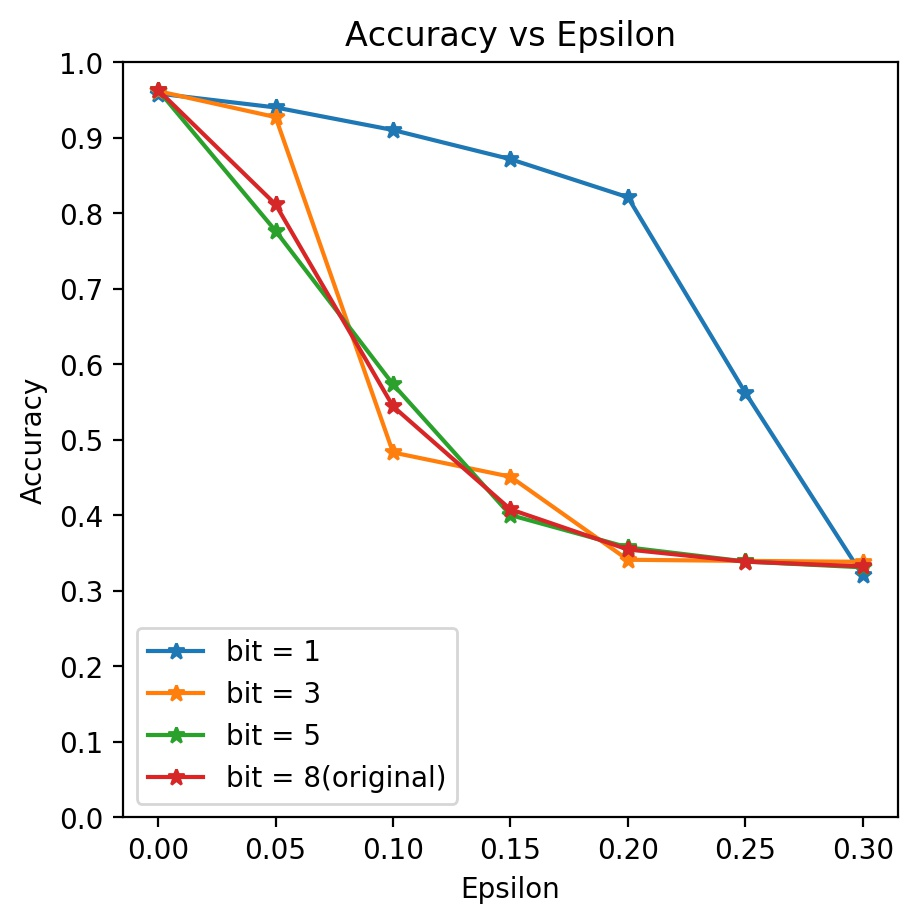
\includegraphics[width=\textwidth]{Accuracy_vs_Epsilon_db.jpg}
		\caption{Our model}
		\label{fig: bit-depth reduction us}
	\end{subfigure}
	\caption{Accuracy for different levels of noise we choose}
\end{figure}



\subsubsection{Total Variation}
\begin{figure}[h!]
	\centering
	\begin{subfigure}{.4\textwidth}
		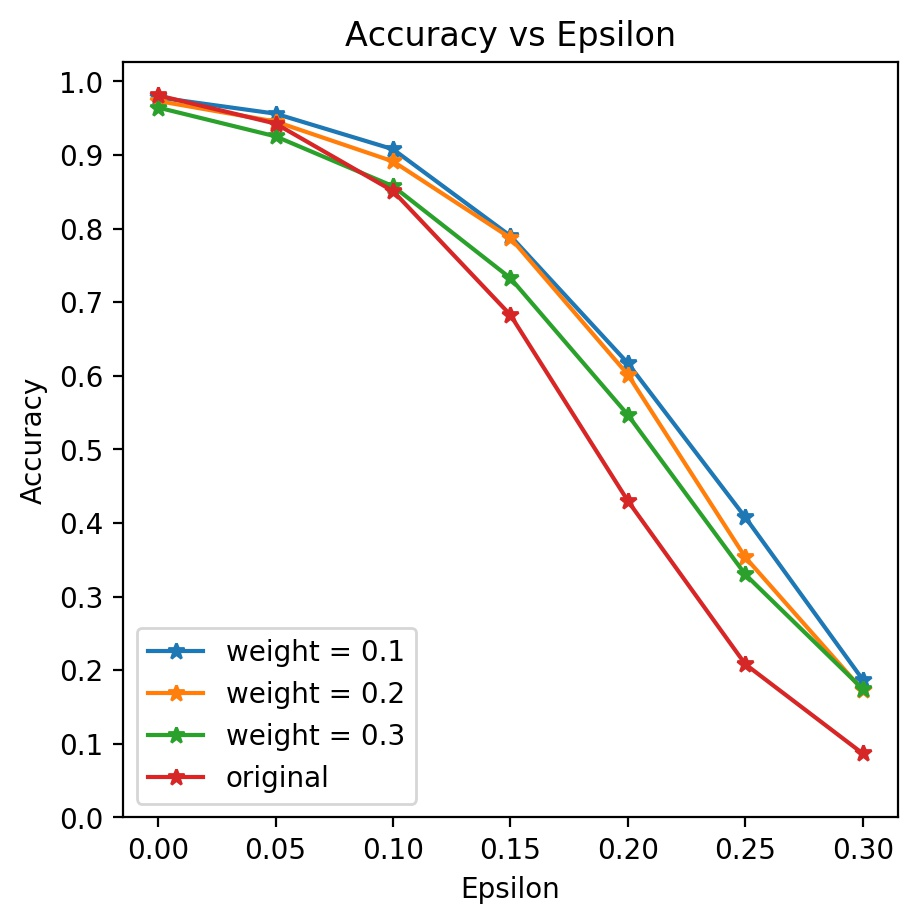
\includegraphics[width=\textwidth]{pretrained_Accuracy_vs_Epsilon_tv.jpg}
		\caption{pretrained model}
		\label{fig: tv pre}
	\end{subfigure}
	\begin{subfigure}{.4\textwidth}
		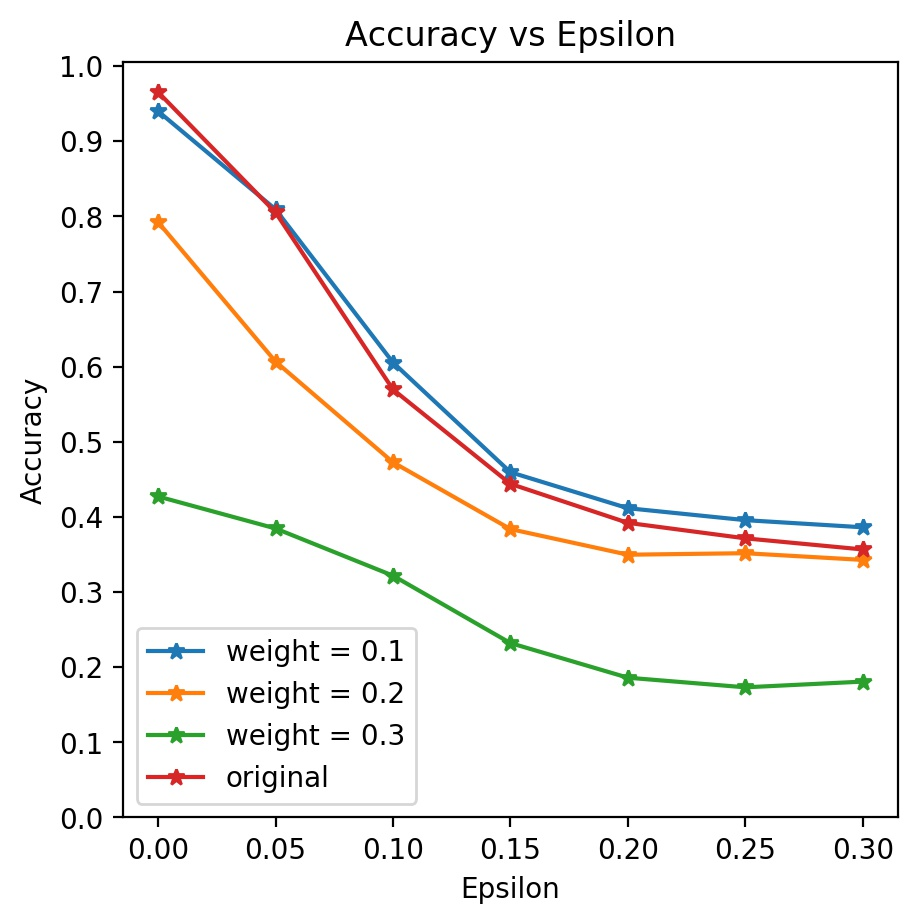
\includegraphics[width=\textwidth]{Accuracy_vs_Epsilon_tv.jpg}
		\caption{Our model}
		\label{fig: tv us}
	\end{subfigure}
	\caption{Accuracy for different levels of noise we choose}
\end{figure}

\subsubsection{Resolution reduction}

As per our description in methods section, we perform two resizing operations on the MNIST dataset. The original images are 28 by 28 pixels, so we scale test images down to 14 by 14, 20 by 20 or 24 by 24, then rescale back to 28 by 28.  We see from Figure \ref{fig:resolution} that this method does not appear to work since the model trained on the original data (with stochastic gradient descent) seems more robust. It can be seen that the accuracy decreases immensely in the 14 by 14 case, suggesting the scale chosen is too extreme to be able to clearly distinguish the class. When the magnitude of \(\epsilon\) is increased to 0.15, the rescaled samples had accuracy no better than random guessing. The poor accuracy could be due to the fact that the boundaries are blurred when we scale down and back-up again, making those regions more sensitive to perturbations, although further investigations could be carried out on other datasets to confirm this.

\begin{figure}[h!]
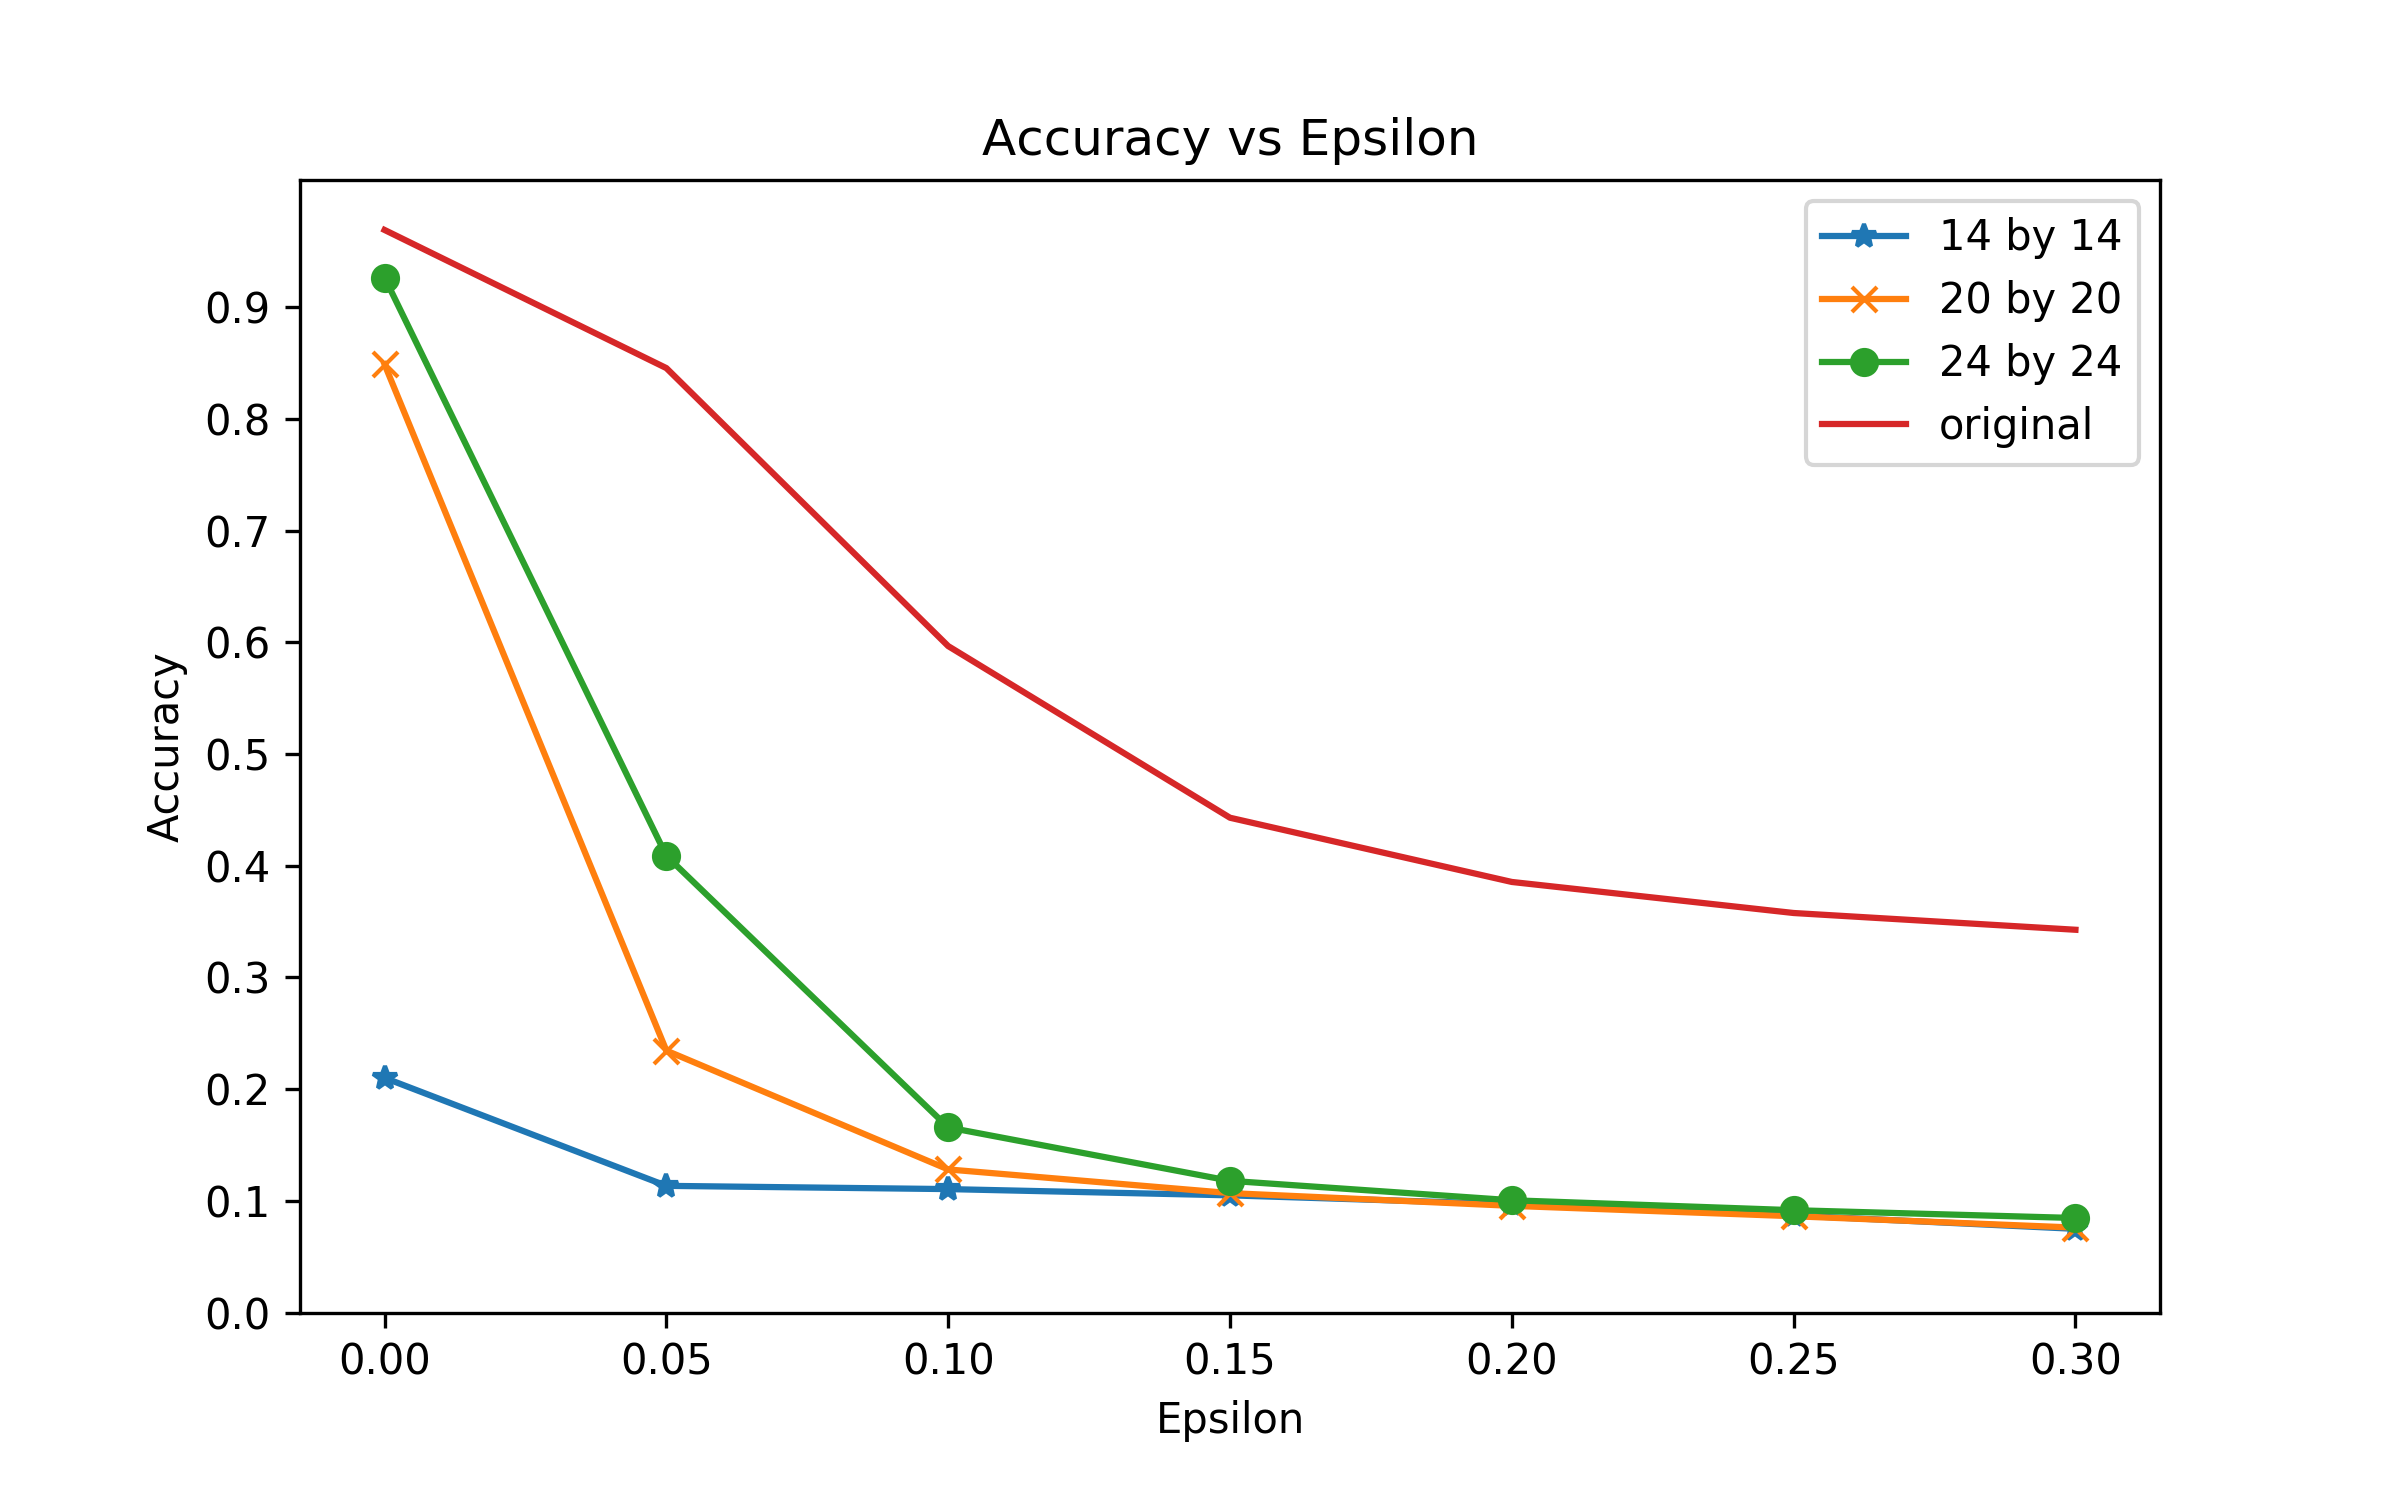
\includegraphics[width=\textwidth]{rescaled_adam}
		\caption{Accuracy in classification under FGSM attacks after a range of rescaling to reduce image resolution.}
		\label{fig:resolution}

\end{figure}

\subsection{Randomised Crop-and-rescale}

We applied 30 randomised crop-and-rescale transformations onto each test subject and then feed all 30 transformed images into the neural network. We record the final classification of the original image as either the mode of the output classes or the class with the highest average sigmoid value across the 30 transformations. The results of such transformations can be seen in Figure \ref{fig:rand}. For lower magnitude of errors using the original test images seem to be better, however the situation is reversed when epsilon increases beyond 0.15. It appears that this method is more robust for perturbations of higher magnitude.

\begin{figure}[h!]
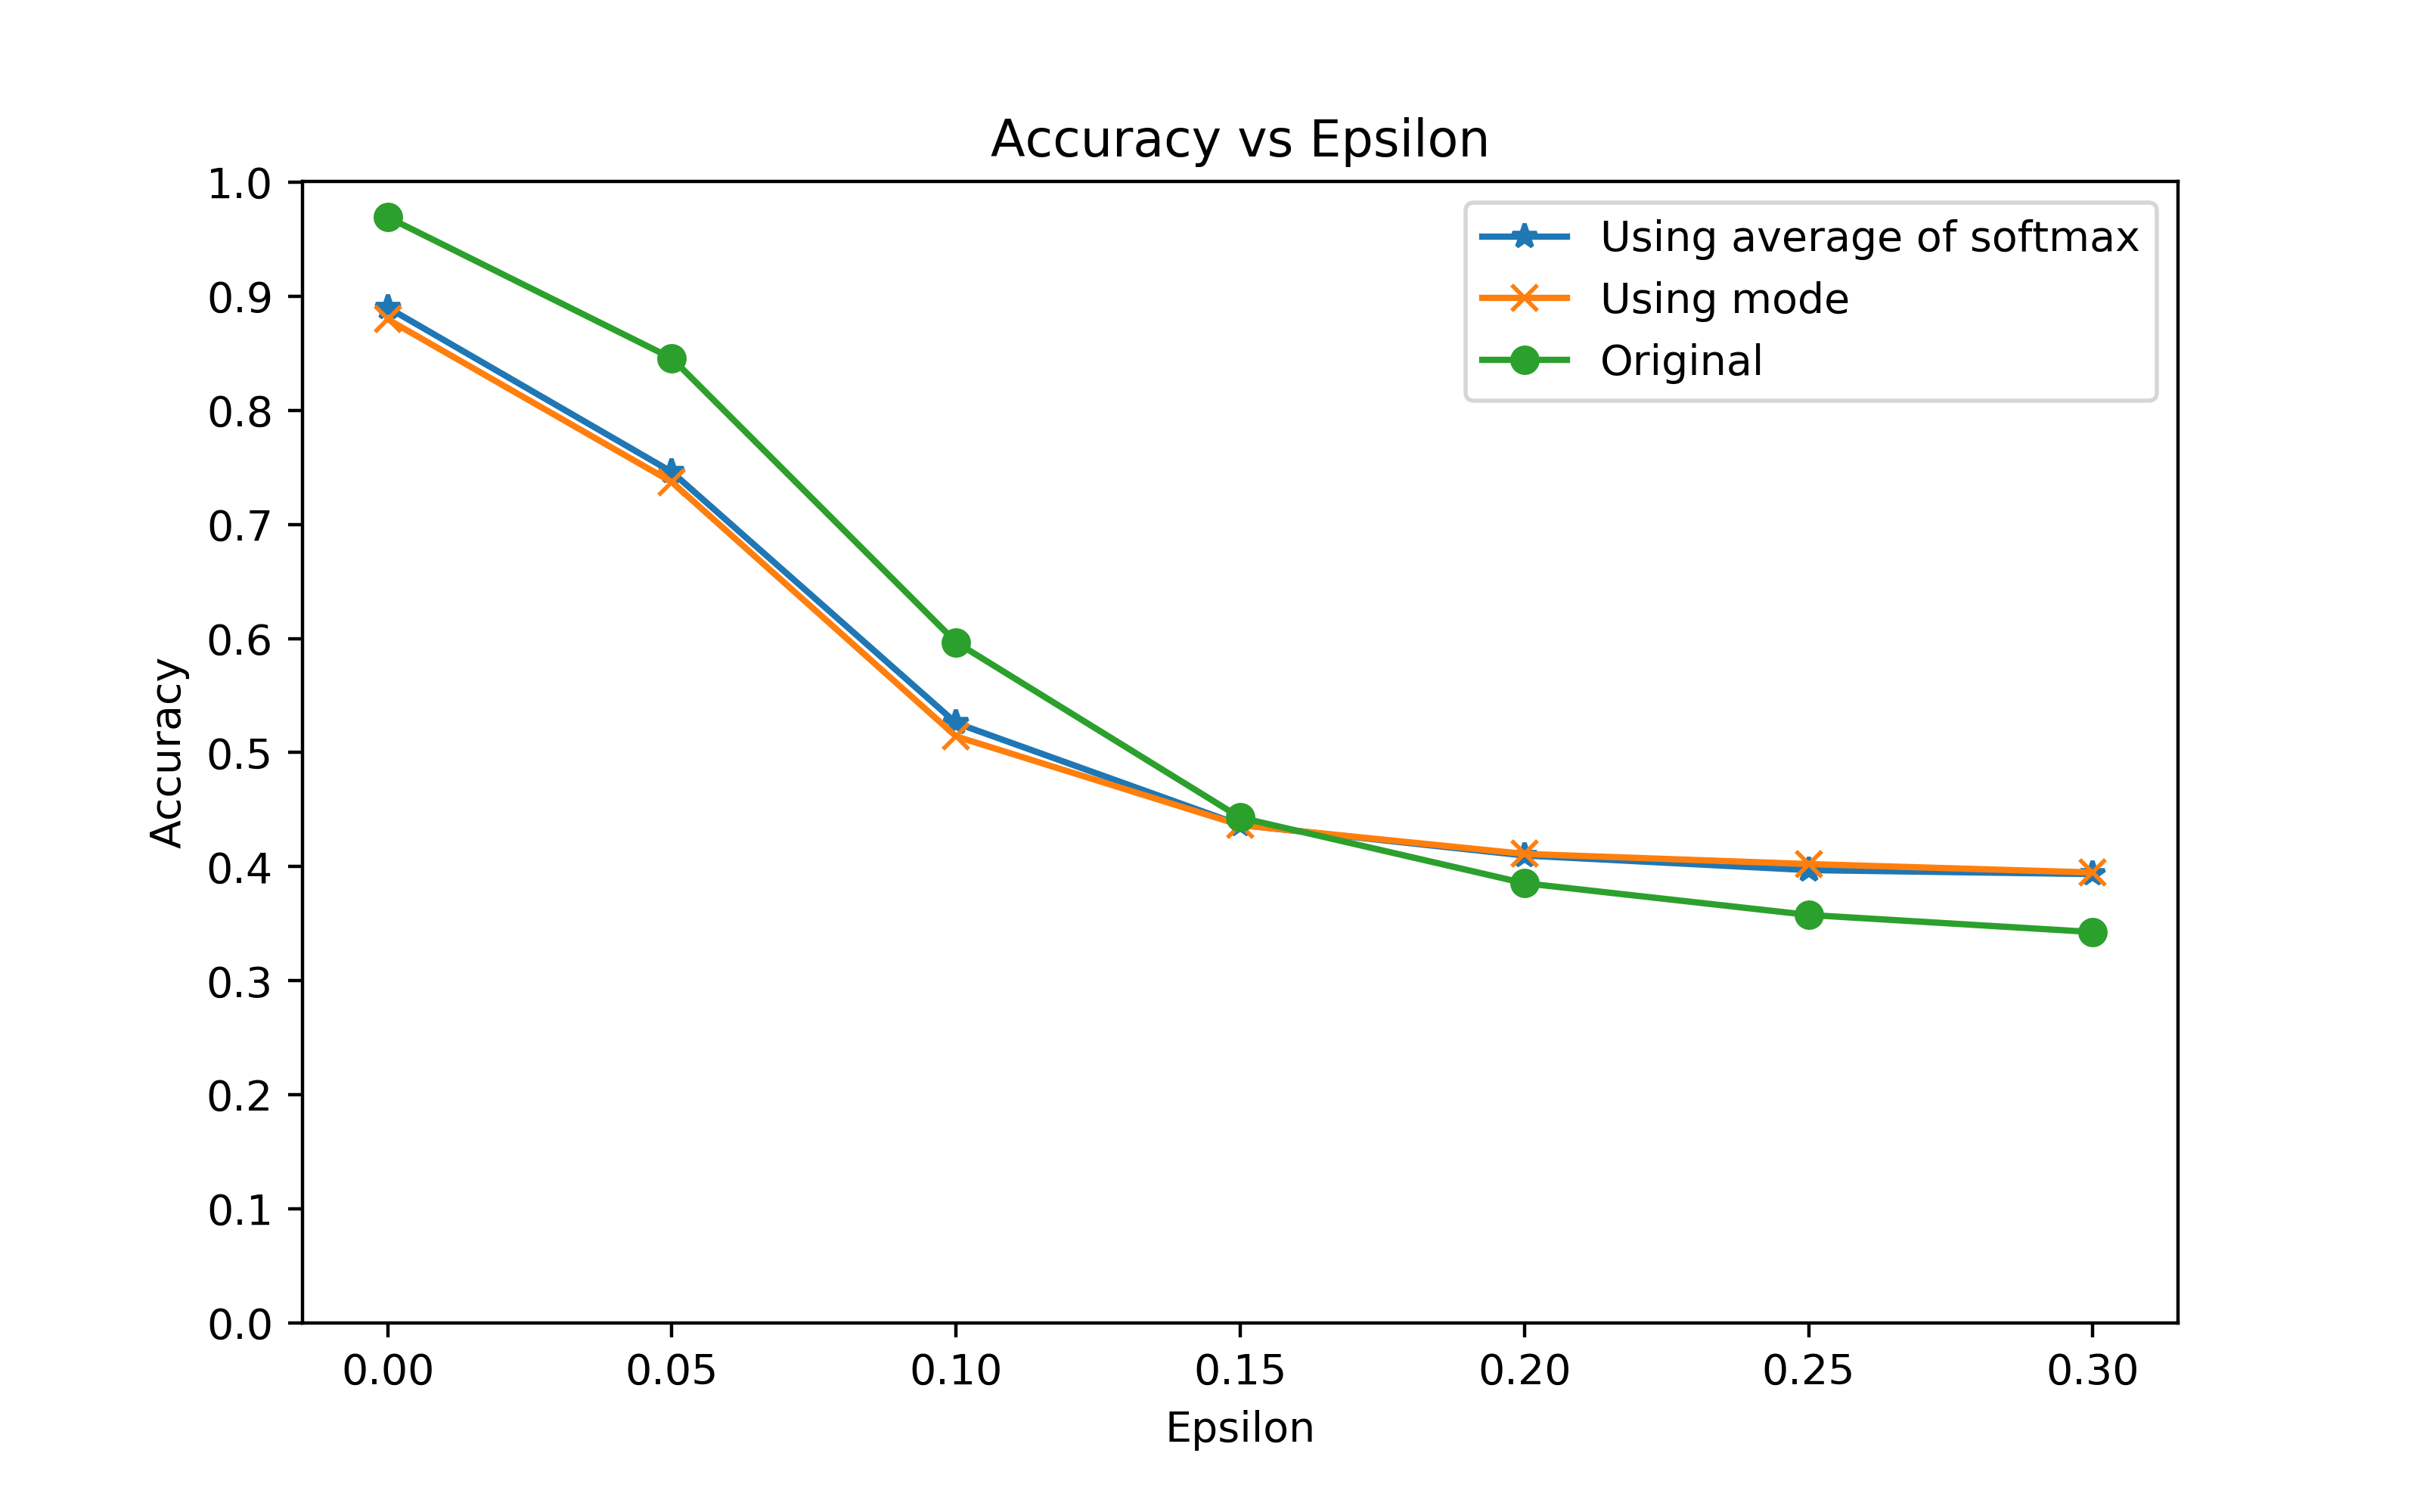
\includegraphics[width=\textwidth]{sgd_random}
		\caption{Accuracy in classification under FGSSM attacks using randomised crop-and-rescale transformations}
		\label{fig:rand}

\end{figure}